\chapter{Results and Discussion}
\label{chapter:results}
Since the data doesn't have labels indicating which entries are anomalies, precise quantitative evaluation is not possible. To examine how the methods perform, user interpretation of the data is the only standard. To help strengthen intuitive understanding, a visualization method t-SNE\cite{maaten2008visualizing} was applied. This method only requires a distance metric between pairs of data entries. Then it projects the entries into a 2D space showing potential structures underlying the data. Information loss is inevitable while projecting high-dimensional data into low dimensional space. t-SNE can't reflect the exact structure of the clusters, still it gives useful information. t-SNE typically places ``important points'' in dense central part of the drawing. The term ``important points'' means points having many near neighbours. So, these points are very likely to locate in dense areas in their original space, too. Intuitively, points lying in dense area are less likely to be outliers. 

Section~\ref{sec:clustering} and ~\ref{sec:generative} describes results obtained using clustering method and generative method respectively. Then, Section~\ref{sec:discuss} compares these two methods.
\section{Clustering Method Results}
\label{sec:clustering}
The first step of applying DBSCAN is to choose parameters. As stated in Section~\ref{subsec:DBSCANalgorithm}, DBSCAN is relatively robust with $k > 4$, where $k$ stands for the $k$th nearest neighbour. In this experiment, $k$ was set to 7. The distance of the $7$th nearest neighbour of all points is draw in Figure~\ref{fig:paramDBSCAN}. The figure shows that the distance begins to increase dramatically beyond 0.5. Thus, in the experiment, $\epsilon$ was finally set to 0.5, with $MinPts = 7$. The clustering result is shown in Table~\ref{tab:ClusterResult} and visualized in Figure~\ref{fig:ClusterResult}.
\begin{figure}[!ht]
	\begin{center}
		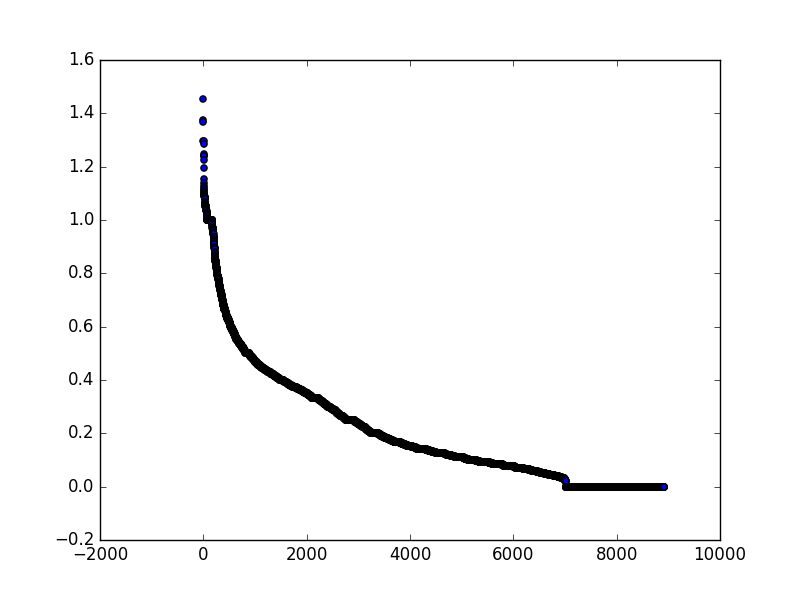
\includegraphics[width=\textwidth]{images/paramDBSCAN}
		\caption{7th nearest neighbour distance for selecting $\epsilon$ of DBSCAN}
		\label{fig:paramDBSCAN}
	\end{center}
\end{figure}

\begin{table}[!ht]
	\caption{Number of points in each cluster generated by DBSCAN.}
	\small
	\begin{center}
		\begin{tabular}{|c|c|c|c|c|c|c|c|c|c|c|c|c|}
			\hline
			Cluster No. &    0 & 1  & 2    & 3   & 4   & 5   & 6  & 7   & 8  & 9  & 10 & 11	\\ \hline
			Num Points  &  352 & 10 & 7547 & 134 & 215 & 283 & 64 & 104 & 44 & 47 & 21 & 94 \\
			\hline

		\end{tabular}
	\end{center}
	\label{tab:ClusterResult}
\end{table}

As shown in the table, 12 clusters are generated by DBSCAN. Among the 12 clusters, cluster 0 is labelled as noise/anomalies which consists of 352 visits. Cluster 2 is the largest cluster which consists of 7547 visits. This cluster is believed to consists of the most typical visits. For the rest small clusters, they can be considered as representing some non-typical but normal visits. One potential reason of generating such sub-clusters is that, there are many different resources/machines for diagnosing. Data in these sub-clusters are generated from these less frequently used resources/machines. The result is visualized in Figure~\ref{fig:ClusterResult}.

\begin{figure}[!ht]
	\begin{center}
		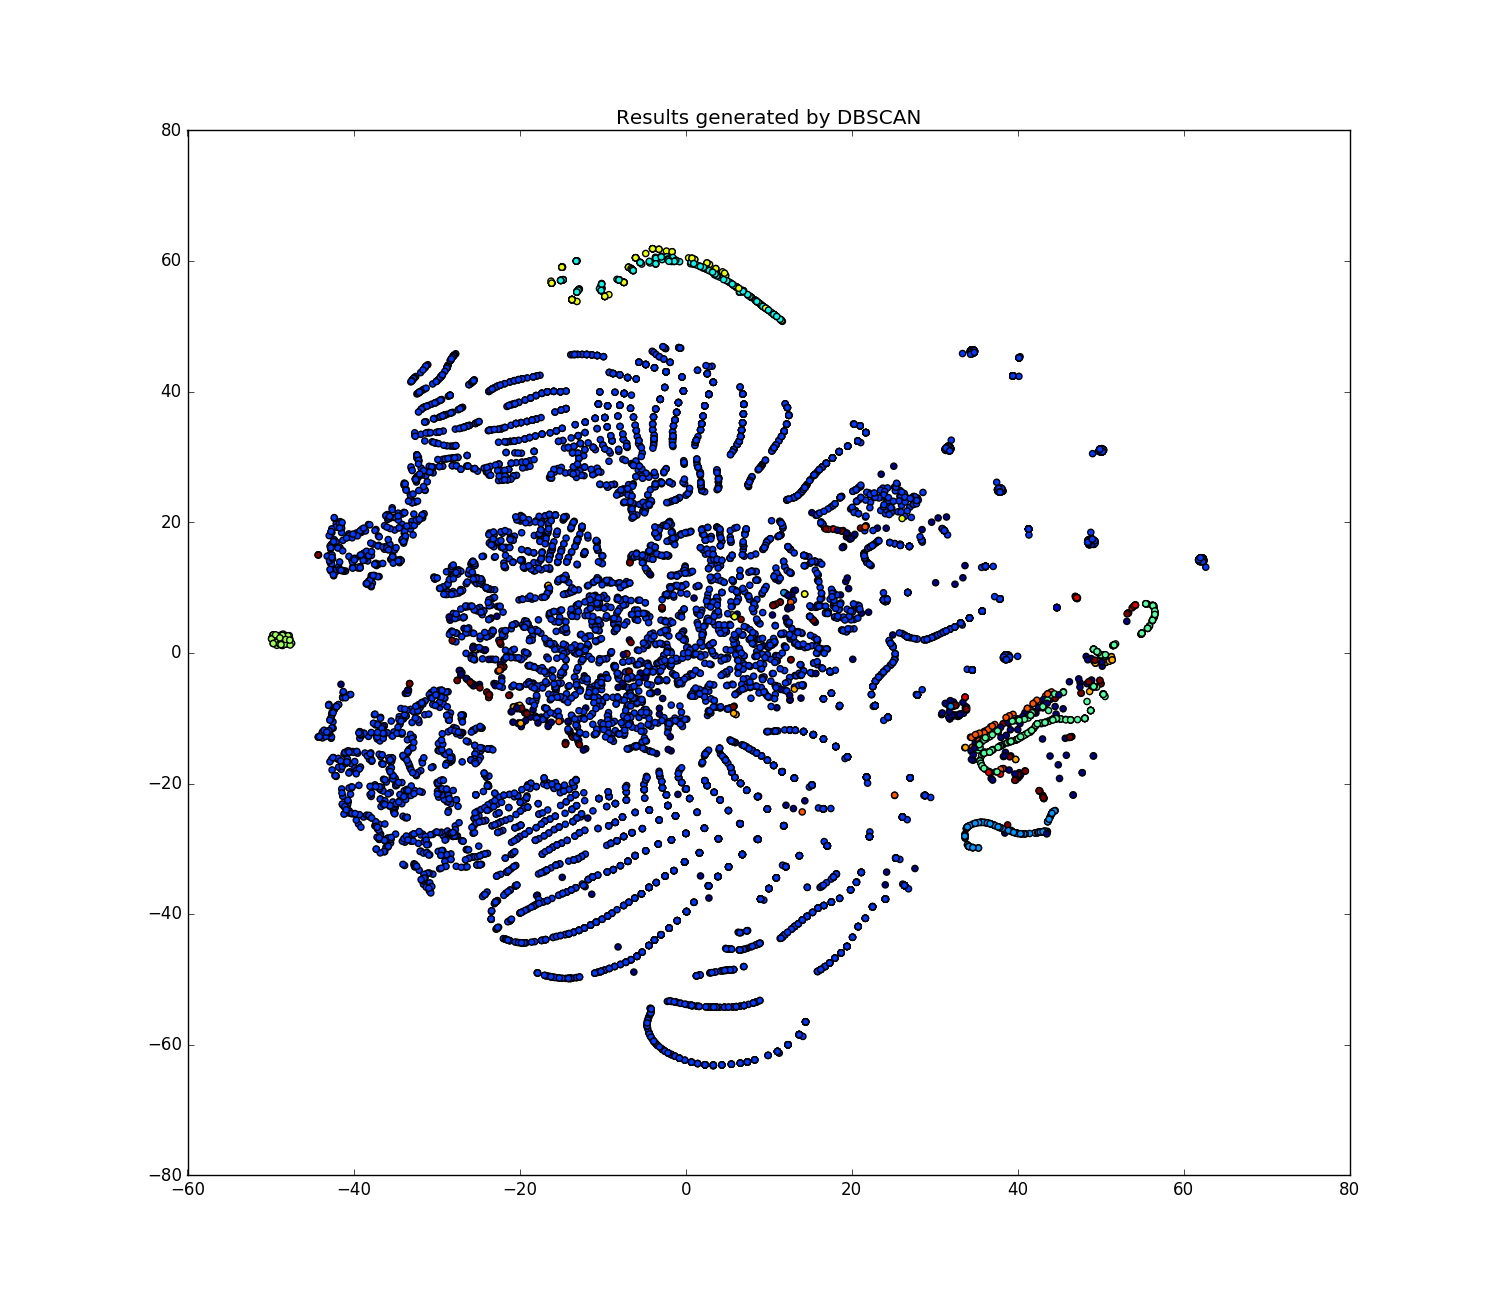
\includegraphics[width=\textwidth]{images/ClusterResult}
		\caption{Results generated by DBSCAN, visualized using t-SNE. All clusters are shown. Each cluster is plotted in a different color.}
		\label{fig:ClusterResult}
	\end{center}
\end{figure}

In Figure~\ref{fig:ClusterResult2}, cluster 0 is plotted using red while the rest clusters are all painted in blue. As the figure shows, many red points located on the border of the figure, which indicates they come from sparse areas in their original space and are more likely to be anomalies. To further verify our suspicion, we went though the visits assigned to each cluster. 10 samples from each cluster are listed in Table~\ref{tab:samplesFromCluster}. 

Visits in Cluster 0 seem very uncommon. Some visits just ended without neither closed by the doctor nor cancelled by the patient. Cluster 1 consists of similar visits. Cluster 2 seems to have many reasonable visits. Visits from this cluster typically consists of four events and each event has duration no longer than 30 minutes. Thus, this cluster can be interpreted as the collection of normal visits as assumed. The rest clusters also exhibit some intuitive patterns. Some small clusters can be also considered as anomalies in addition to cluster 0, for example, cluster 10. The reason there are many clusters is that the distance between border points in two clusters are too large so that the two clusters did not merge. 

\begin{figure}[!ht]
	\begin{center}
		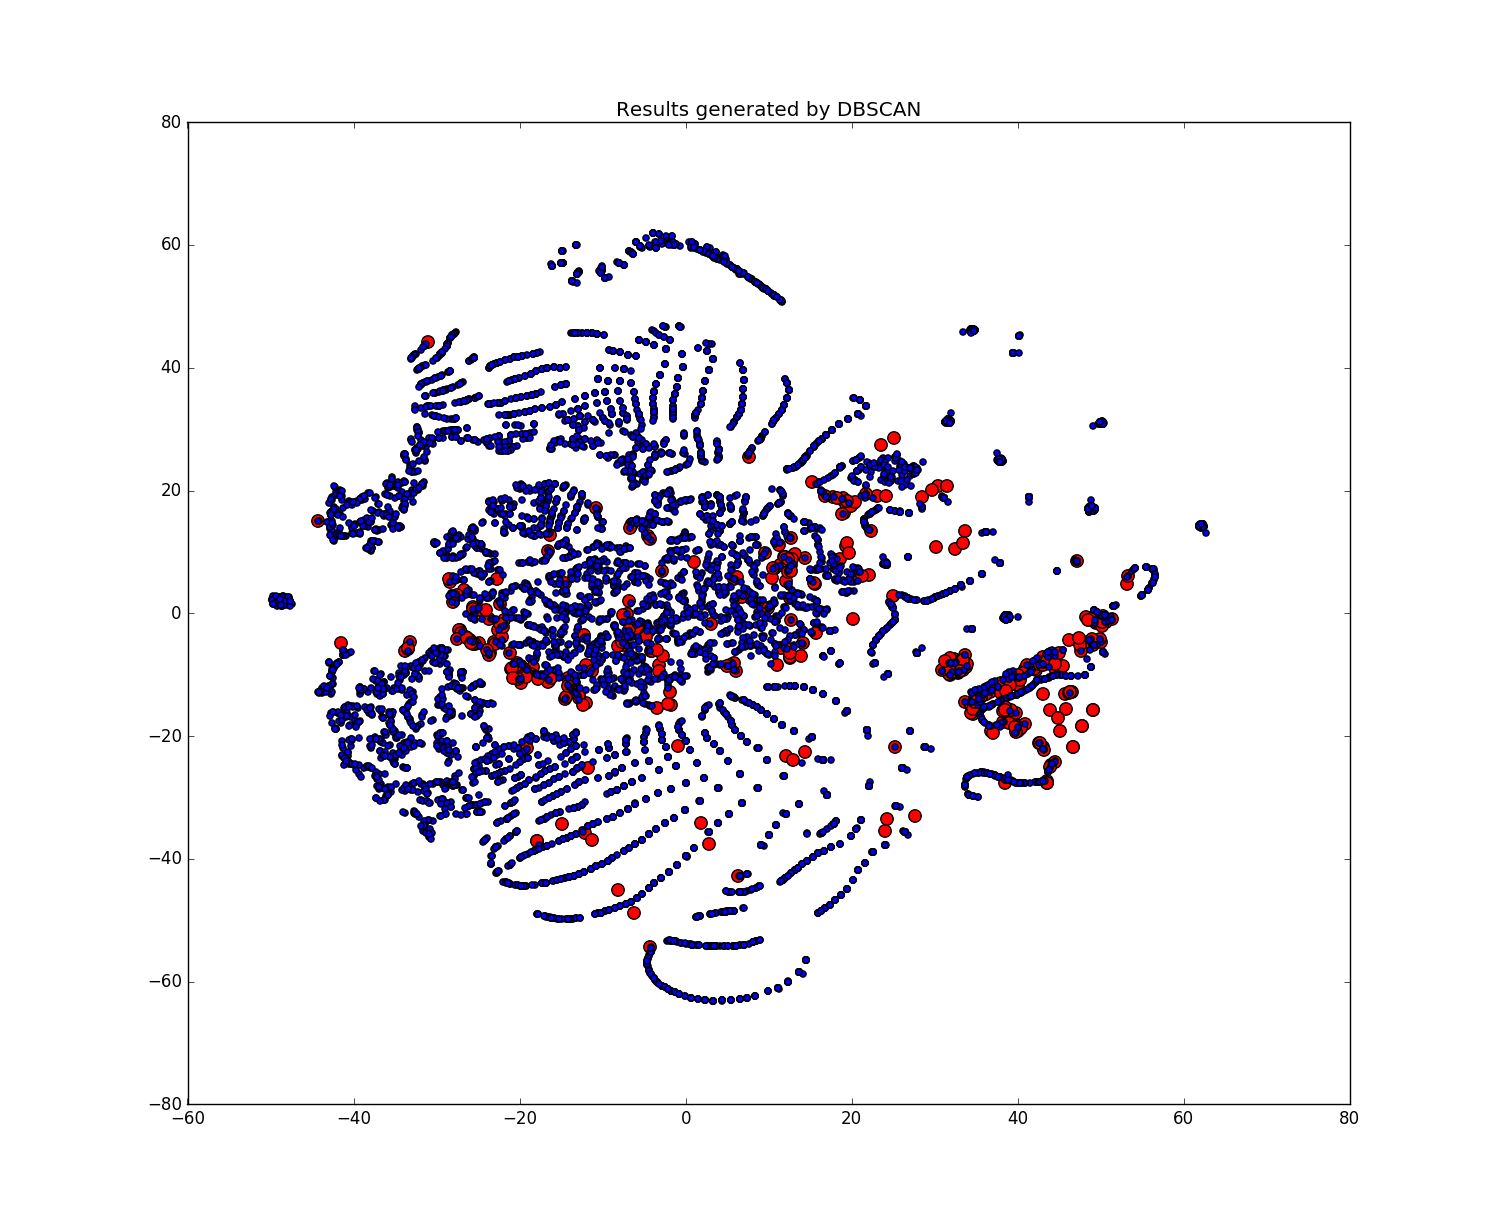
\includegraphics[width=\textwidth]{images/ClusterResult2}
		\caption{Results generated by DBSCAN, visualized using t-SNE. Cluster 0 are represented by enlarged red points, while all the rest clusters are represented by blue points. Notice that red points mainly locate in sparse areas, which suggests they are more likely to be anomalies. However, some red points also appear in dense areas, which are less likely to be anomalies. This suggests that the results generated by DBSCAN may have some errors.}
		\label{fig:ClusterResult2}
	\end{center}
\end{figure}

However, we also notice that some red points appear in dense areas. As we mentioned, points appeared in dense areas tend to be ``important''. This observation suggests that the DBSCAN algorithm may have labelled some normal points as anomalies. For example, the last sample visit in cluster 0 is not a typical normal visit, but it could still be considered as normal. In fact, as we went through all visits assigned to cluster 0, we indeed found some normal visits.

\section{Generative Method Results}
\label{sec:generative}
Compared to DBSCAN, Markov Chain method is easier to implement. However, some special rules need to be set before running the method. The first rule is how to handle the -1 appeared in each event, which means the visit terminates. Since negative binomial only defines probability for non-negative inputs, the probability of duration equals -1 is undefined. In the experiment, we set this probability to be the frequency of being -1 happened in this event. This makes the summation of the probability of all possible values slightly larger than 1. However, we can easily fix the problem by scaling.

Another caveat is the numerical issues while computing likelihood. Since the likelihood of a probability will typically be so small that precision problem may occur. To avoid this, the log-likelihood is computed instead. Visits having longer sequence of events tend to have smaller likelihood, but this does not mean the visit is less likely to happen. Considering this problem, the final log-likelihood is normalized by dividing the length of the sequence. The log-likelihood of visits sorted in decreasing order is shown in Figure~\ref{fig:likelihood}. As shown by the figure, most visits have a log-likelihood larger than -10, the rest few visits with log-likelihood much smaller than -10 are very like to be anomalies. After selecting a threshold to be -10, the detection result is shown in Figure~\ref{fig:MarkovResult}. Anomalies are painted in red. Again, these suspected anomalies locates on border areas in the figure.

Similarly, for every 1000 visits, 5 samples are selected with their log-likelihood listed in Table~\ref{tab:samplesFromGenerative} for further exploration. As listed in the table, visits in the first several blocks are very similar and seem to be very normal. It was only from the last but one block, visits start to behave in different ways. And in the last block, which consists of visits have very large negative values of log-likelihood, these visits are very bizarre and are exactly the anomalies we tried to find.


\begin{figure}[!ht]
	\begin{center}
		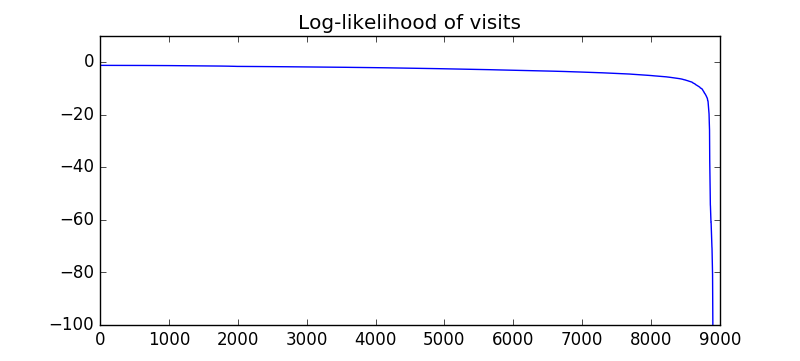
\includegraphics[width=\textwidth]{images/likelihood}
		\caption{Log-likelihood of all visits sorted in decreasing order.}
		\label{fig:likelihood}
	\end{center}
\end{figure}

\begin{figure}[!ht]
	\begin{center}
		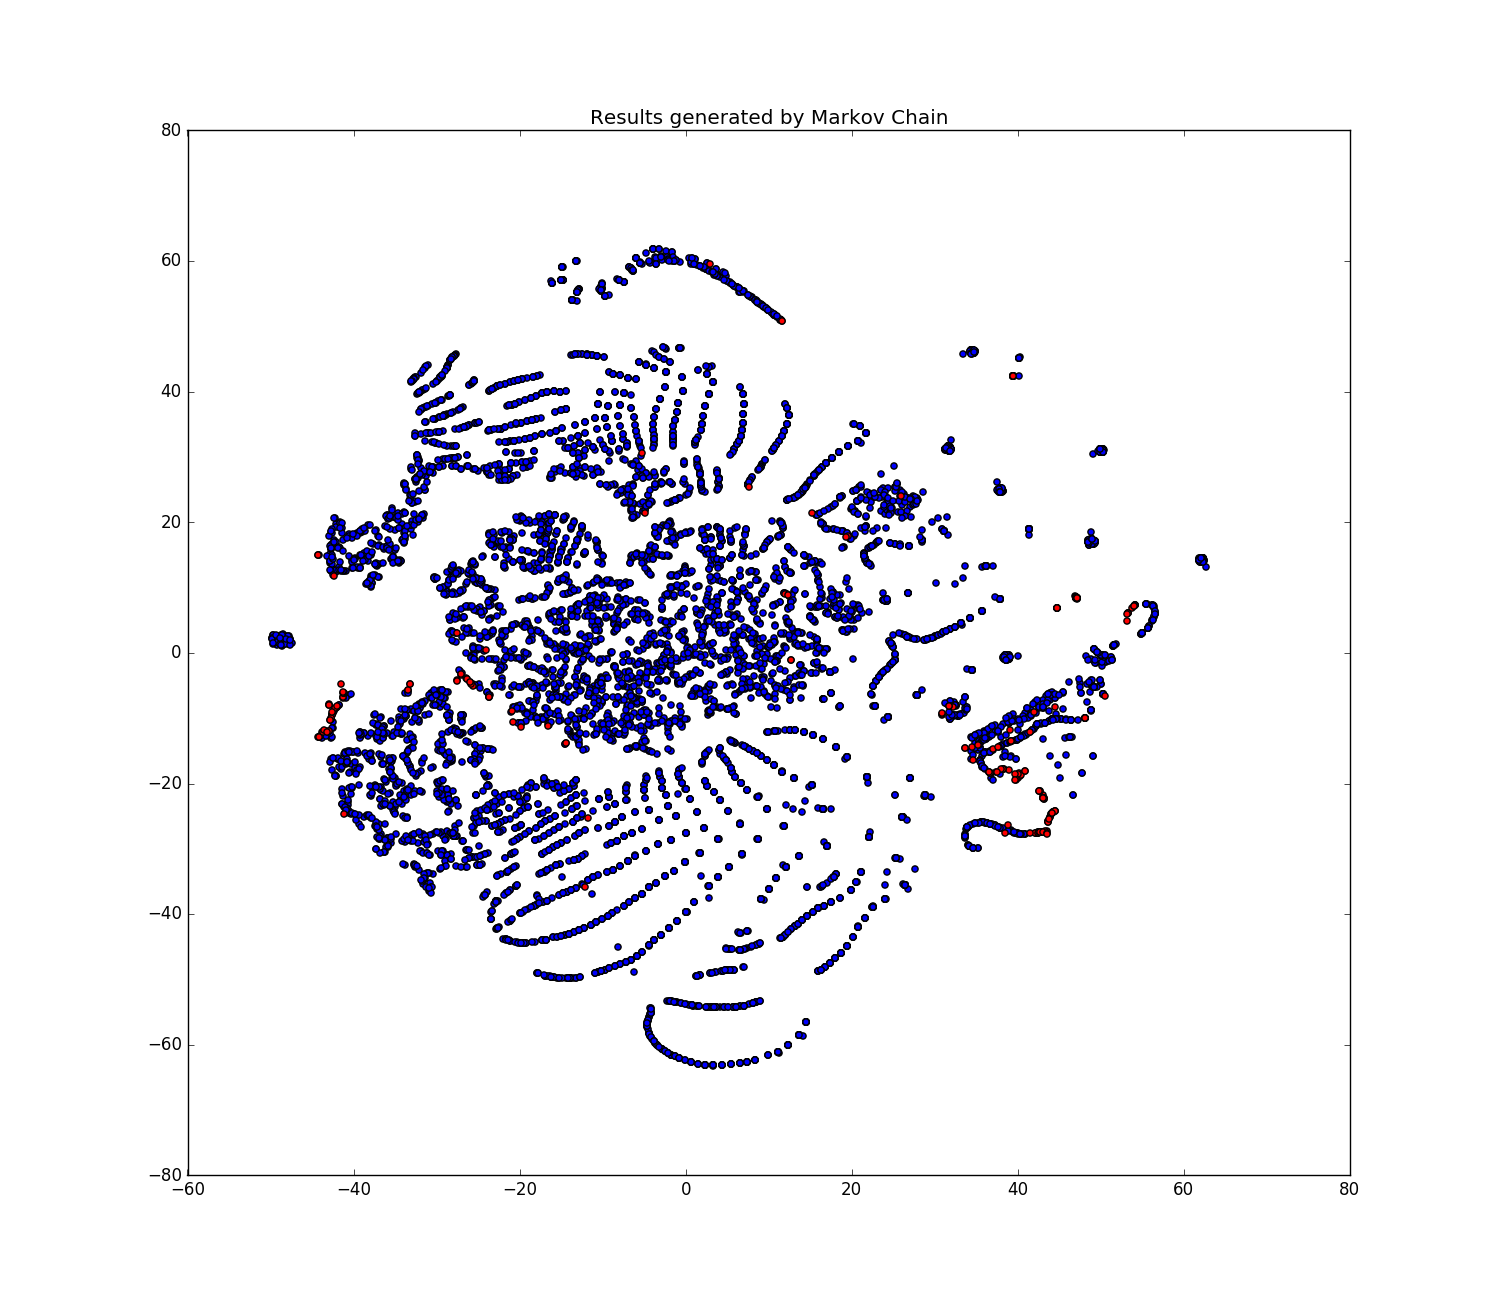
\includegraphics[width=\textwidth]{images/MarkovResult}
		\caption{Results generated by first-order Markov Chain using negative binomial distribution as emission function, visualized using t-SNE. Anomalies are indicated by enlarged red points. Notice that, again red points mainly locate in sparse areas, which suggests they are more likely to be anomalies. Compared to Figure~\ref{fig:ClusterResult2}, much less red points appear in dense areas.}
		\label{fig:MarkovResult}
	\end{center}
\end{figure}

\section{Discussion}
\label{sec:discuss}
Above result suggests both DBSCAN and Markov Chain can spot out anomalies. However, compared to DBSCAN, we think Markov Chain is a better method for several reasons. 

Firstly, clusters formed by DBSCAN are slightly contaminated. For example, the 4th visit in cluster 7 seems very abnormal and should appear in other clusters. Other clusters also have entries does not resemble other visits in this log. A reason for such behaviour is the hard assignment to clusters in DBSCAN. In Markov Chain, however, each visit is assigned by a score which indicates how ``normally'' this visit is. This ``soft-assignment'' is a better description of the entries. Besides, the user has to interpret the meaning of each cluster by themselves, which is typically unexpected by the user.

Secondly, Markov Chain has better time and space complexity for detecting future anomalies. When determining if a new visit log is anomaly, DBSCAN will compare this new visit to all past visits and then assign this new visit to the cluster fitting it best. Thus, DBSCAN requires to maintain all past visits, and new detection takes $O(n)$ time. This requirement will gradually becomes impractical. In contrast, Markov Chain only needs to maintain the computed parameters of transition matrix and emission functions. Computing the log-likelihood takes $O(1)$ time for each new visit log. Thus, speaking from this aspect, Markov Chain is a much better method than DBSCAN.